% Author: Emmanuel D. Solis
\documentclass{article}

% Set font encoding for PDFLaTeX, XeLaTeX, or LuaTeX
\usepackage{ifxetex,ifluatex}
\if\ifxetex T\else\ifluatex T\else F\fi\fi T%
  \usepackage{fontspec}
\else
  \usepackage[T1]{fontenc}
  \usepackage[utf8]{inputenc}
  \usepackage{lmodern}
\fi

%--------- Bibliografias --------
\usepackage{apacite} %Trabajar bibliografias APA
\usepackage{natbib} %Agregar Bibliografias

%------------ Estilos -----------
\usepackage{afterpage} %Agregar paginas en blanco
\usepackage{bookmark} %Para bookmark del indice
\usepackage[shortlabels]{enumitem} %Para enumerar con letras
\usepackage{float} %Tablas y posicionamiento de figuras.
\usepackage{fullpage} %Trabajar con menos margenes de pagina
\usepackage{graphicx} %Agregar imagenes
\usepackage{hyperref} %Uso de vinculos
\usepackage{pdfpages} %Incluir pdf externos
\usepackage{xcolor}  %Usar colores

%---------- Herramientas ----------
\usepackage{amsfonts} %Formulas matematicas
\usepackage{amsmath} %Alinear ecuaciones y similar.
\usepackage{listings} %Comandos de Terminal UNIX.
\usepackage{minted} %Incluir codigo de programacion.
%\usepackage{sagetex} %Hacer calculos
\usepackage{venndiagram} %Agregar diagramas de Venn

%----------- Idiomas ---------------
\usepackage[spanish]{babel} %Configurar el idioma

\begin{document}

\begin{titlepage}
\centering
{
\includegraphics[width=0.2\textwidth]{logoUCR.png}\par}
\vspace{1cm}
{\bfseries\LARGE Universidad de Costa Rica \par}
\vspace{1cm}
{\scshape\Large Facultad de Ingenier\'ia \par}
{\scshape\Large Escuela de Ciencias de la Computaci\'on e Inform\'atica \par}
\vspace{1cm}
{\scshape\Large CI0128 – Proyecto Integrador: Ingeniería de Software y Bases de Datos \par}
{\scshape\Large Profesoras: Rebeca Obando y Alexandra Martínez \par}
\vspace{1cm}
{\scshape\Huge Documentación del Sprint 0 \par}
\vspace{1cm}
{\Large Nombre del Equipo: Ta' Bueno \par}
\vspace{0.5cm}
{\Large Miembros: \par}
{\Large Emmanuel D. Sol\'is - B97670 (Scrum Master)\par}
{\Large \textit{\color{blue}emmanuel.solispomares@ucr.ac.cr} \par}
{\Large Gabriel Zúñiga - B98755\par}
{\Large \textit{\color{blue}gabriel.zunigaorozco@ucr.ac.cr} \par}
{\Large Jan Murillo - B95447\par}
{\Large \textit{\color{blue}jan.murillo@ucr.ac.cr} \par}
{\Large Kevin Arguedas - B80626\par}
{\Large \textit{\color{blue}kevin.arguedasmuriel@ucr.ac.cr} \par}
{\Large Luis D. Chinchilla - B82227\par}
{\Large \textit{\color{blue}luis.chinchillaotarola@ucr.ac.cr} \par}
\end{titlepage}

\newpage
\tableofcontents

\newpage
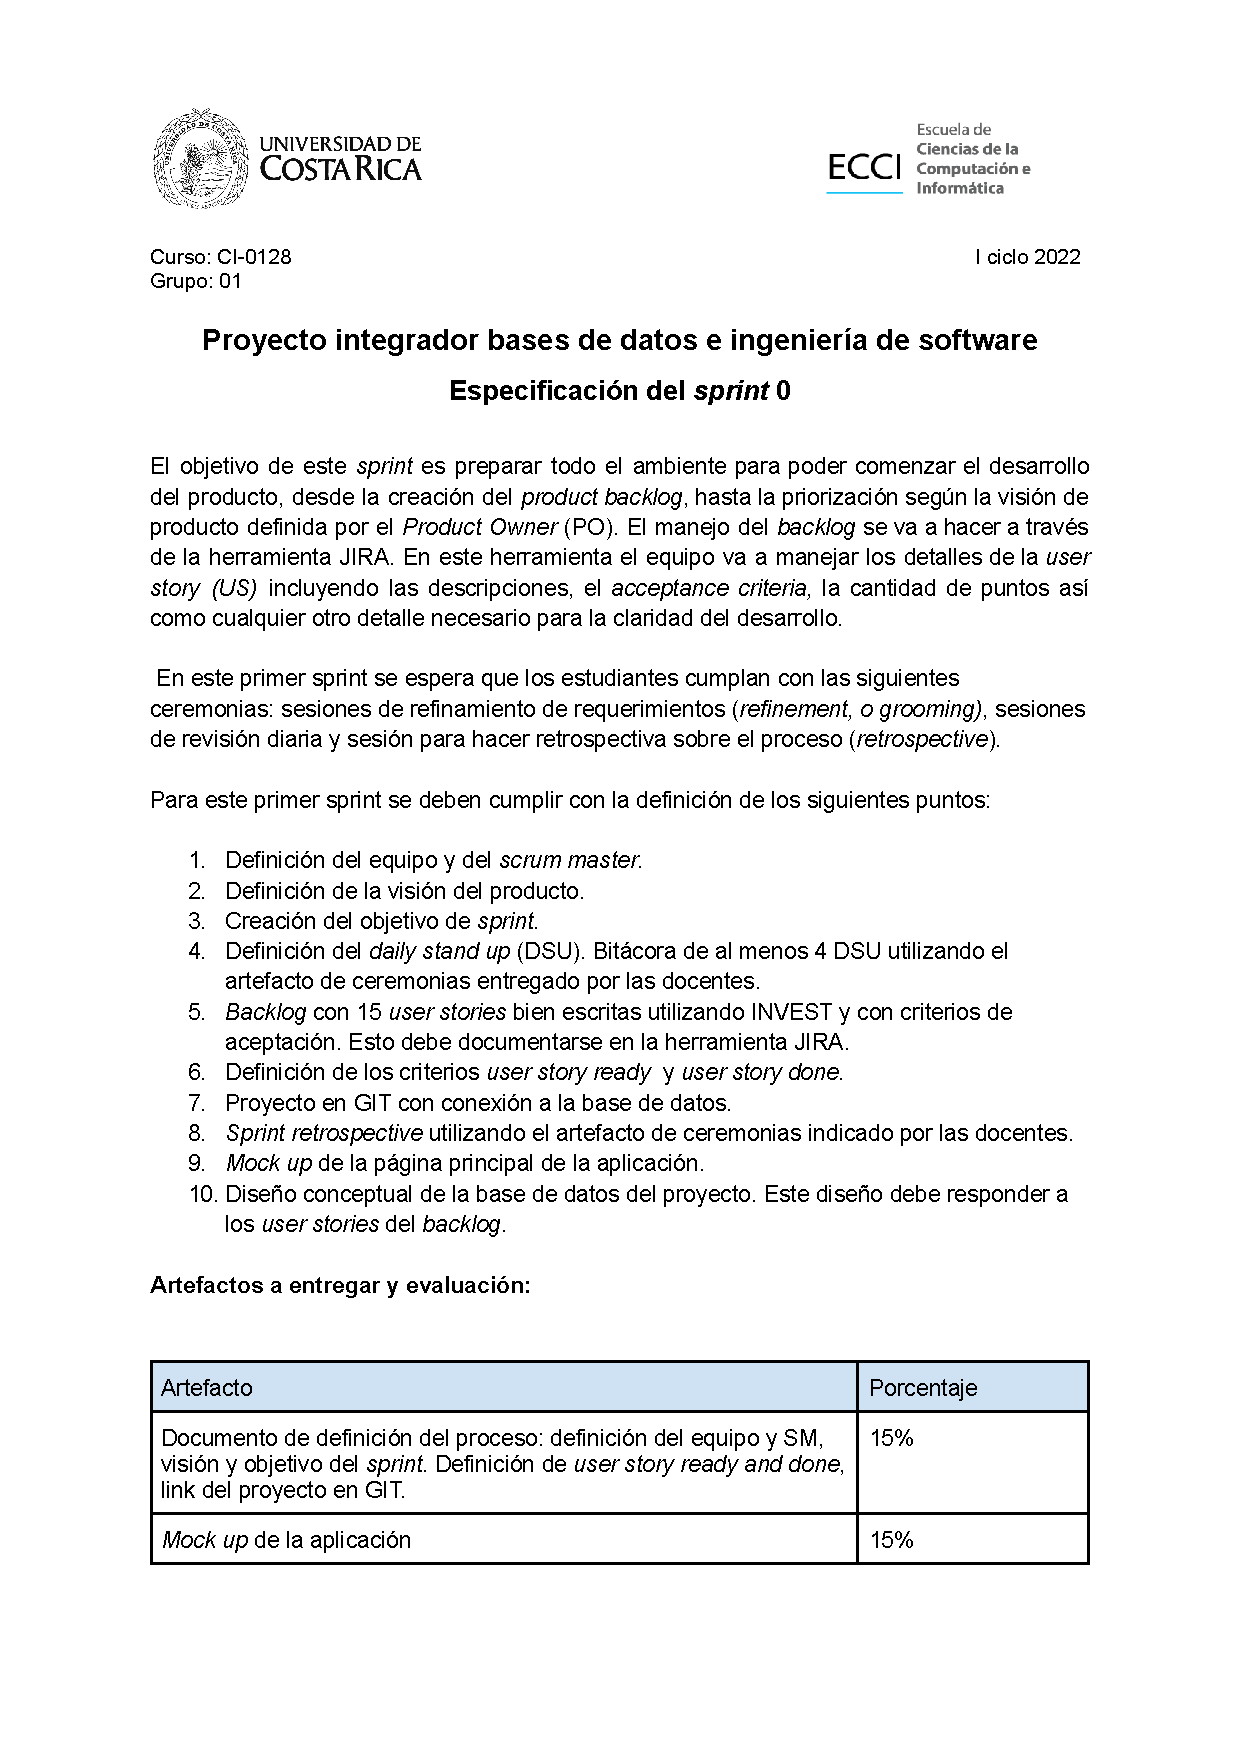
\includepdf[pages={-}]{enunciado.pdf}

\newpage
\section{Definición del equipo y del scrum master}
Nuestro equipo estará conformado por lo siguientes miembros:
\begin{itemize}
  \item Nombre: Emmanuel D. Solis.\\Carné: B97670.
  \item Nombre: Gabriel Zúñiga.\\Carné: B98755.
  \item Nombre: Jan Murillo.\\Carné: B95447.
  \item Nombre: Kevin A. Muriel.\\Carné: B80626.
  \item Nombre: Luis D. Chinchilla.\\Carné: B82227.
\end{itemize}
En la primer sesión, la cuál está corroborada en la sección
Bitácora, se acordó que \textbf{Emmanuel D. Solís} sería el \textbf{Scrum Master}
y \textbf{Jan Murillo} sería la persona encargada de llevar las \textbf{bitácoras}.

\section{Definición de la visión del producto}
Por medio de este sistema de planillas queremos tener un sistema que sea
una ayuda para los empleadores, donde puedan registrar a sus distintos tipos
de empleados y puedan tener en un mismo lugar control de todo lo relacionado
al pago de sus empleados; como beneficios, rebajos de ley, desglose de salarios,
y donde los empleados pueden incluso registrar tiempo trabajado; pretende
ser una herramienta tanto para el empleador como para los empleados, así
estos también tendrán control de saber qué están recibiendo cada fecha de pago
y podrán consultar su historial de pagos.

\section{Creación del objetivo de sprint}
El objetivo de este sprint se centra en la introducción al proyecto y
comprende desde la creación del product backlog hasta la priorización
según la visión de producto definida por el \textit{Product Owner (PO)}.
El manejo del backlog se va a hacer a través de la herramienta \textit{JIRA}.
En esta herramienta el equipo va a manejar los detalles de la
\textit{user story (US)} incluyendo las descripciones, el acceptance
criteria, la cantidad de puntos, entre otros posibles detalles. En este
primer sprint se espera cumplir con las siguientes ceremonias: sesiones
de refinamiento de requerimientos (\textit{refinement, o grooming}),
sesiones de revisión diaria y sesión para hacer retrospectiva sobre el
proceso (retrospective). A su vez, el sprint también tiene como objetivo
dar una vista preliminar (\textit{mock up}) del aspecto de la página principal de
la aplicación web y crear el modelo de la base de datos, derivada de las
\textit{user story} con el fin de preparar el ambiente para poder comenzar
el desarrollo del producto que dará inicio en el \textit{sprint 1}. 

\section{Bitácora}
Podemos ver la bitácora a continuación:

\section{Backlog}
Este se encuentra en la plataforma Jira en el siguiente enlace:
\url{https://ingesoftg001.atlassian.net/jira/software/projects/TB/boards/5/backlog}.

\section{Criterios \textit{user story ready y user story done}}

\section{Proyecto de Git}
El enlace a nuestro repositorio, que se encuentra en GitHub, es
\url{https://github.com/emasp2001/pi_ingeBases.git}. Cabe señalar que
aunque el proyecto es privado ambas profesoras y el asistente han sido
agregados como colaboradores de dicho repositorio por lo que no debería
haber problemas de acceso.

\section{Sprint retrospective}

\section{\textit{Mock up} de la página principal de la aplicación}

\section{Diseño conceptual de la base de datos del proyecto}

%\begin{figure}[h]
%  \centering
%  \includegraphics[width=0.65\textwidth]{SystemCalls.png}
%  \caption{Funcionamiento interno de una interrupción al Sistema Operativo \cite[]{whatSysCalls}.}
%  \label{fig:HowWorksSysCalls}
%\end{figure}

%---------------------- Document Ending ----------------------------------
\newpage
\bibliographystyle{apacite}
\bibliography{bibliography.bib}
\end{document}
